\documentclass[review]{elsarticle}

\usepackage{lineno,hyperref}
\usepackage{rotating}
\usepackage{adjustbox}
\modulolinenumbers[5]
\usepackage{amssymb}
\usepackage{multirow}
\usepackage{amsmath}
\usepackage{subfig}
\journal{Journal of Information Sciences}

%%%%%%%%%%%%%%%%%%%%%%%
%% Elsevier bibliography styles
%%%%%%%%%%%%%%%%%%%%%%%
%% To change the style, put a % in front of the second line of the current style and
%% remove the % from the second line of the style you would like to use.
%%%%%%%%%%%%%%%%%%%%%%%

%% Numbered
%\bibliographystyle{model1-num-names}

%% Numbered without titles
%\bibliographystyle{model1a-num-names}

%% Harvard
%\bibliographystyle{model2-names.bst}\biboptions{authoryear}

%% Vancouver numbered
%\usepackage{numcompress}\bibliographystyle{model3-num-names}

%% Vancouver name/year
%\usepackage{numcompress}\bibliographystyle{model4-names}\biboptions{authoryear}

%% APA style
%\bibliographystyle{model5-names}\biboptions{authoryear}

%% AMA style
%\usepackage{numcompress}\bibliographystyle{model6-num-names}

%% `Elsevier LaTeX' style
\bibliographystyle{elsarticle-num}
%%%%%%%%%%%%%%%%%%%%%%%

\begin{document}

\begin{frontmatter}
\title{Semi-supervised Multi-task Learning Using Convolutional AutoEncoder for Faulty Code Detection with Limited Data}
% \title{Elsevier \LaTeX\ template\tnoteref{mytitlenote}}
% \tnotetext[mytitlenote]{Fully documented templates are available in the elsarticle package on \href{http://www.ctan.org/tex-archive/macros/latex/contrib/elsarticle}{CTAN}.}

%% Group authors per affiliation:
\author{Anh Phan Viet \corref{mycorrespondingauthor}}
\ead{anhpv@lqdtu.edu.vn}
\author{Khanh Nguyen Duy Tung}
\author{Lam Bui Thu}
\address{Le Quy Don Technical University, 236 Hoang Quoc Viet St., Hanoi, Vietnam}
% \fntext[myfootnote]{Since 1880.}

% %% or include affiliations in footnotes:
% \author[mymainaddress,mysecondaryaddress]{Elsevier Inc}
% \ead[url]{www.elsevier.com}

% \author[mysecondaryaddress]{Global Customer Service\corref{mycorrespondingauthor}}
\cortext[mycorrespondingauthor]{Corresponding author}

% \address[mymainaddress]{1600 John F Kennedy Boulevard, Philadelphia}
% \address[mysecondaryaddress]{360 Park Avenue South, New York}

\begin{abstract}
This paper proposes a semi-supervised multitask learning framework to overcome the limited data problem for faulty code prediction. The framework has two parts including 1) a convolutional autoencoder performing the auxiliary task that is learning the latent representations of programs and 2) a sequence-based convolution for the main task of faulty code prediction. The keys to reduce the data requirement and remain the prediction accuracy are 1) latent representations can support to generate good features for the classification task and 2) pretraining the joining part with the unsupervised procedure and then fine-tuning with labeled data instead of training from scratch. To evaluate the benefits of pretraining and latent representations, we tried to feed the model with different amount of labelled data. Our experiments on four real datasets of software fault prediction have shown that pretrained the autoencoder achieves better performance and multitask learning makes the model able to learn with limited labelled data. Specifically, the model was trained with 50\% or 70\% can reach the performance as trained with 100\% of data.     
\end{abstract}

\begin{keyword}
Faulty Code Detection \sep Semi-supervised Learning \sep Multi-task Learning \sep Convolutional AutoEncoder 
\end{keyword}

\end{frontmatter}

\linenumbers

\section{Introduction}
\label{sec:introduction}
Detecting faulty modules before releasing projects is crucial to software industry. Faulty code contains specific bugs, e.g. division by zero, infinite loops and buffer overflow that make programs work incorrectly such as out of memory, execution interruption, or generating the unexpected output. It is infeasible to prevent all bugs in software components due to various causes including programmer's skill, miscommunication, buggy third-party tools and so on. According to annual reports, software bugs have led to many devastating consequences in terms of the loss of finance, company reputation and customer satisfaction \cite{laradji2015software}. The later the bugs are detected in the development process, the more serious the consequences are. For above reasons, faulty code detection (FCD) is a hot topic for both academia and industry in the field of software engineering.

There are two major approaches to build machine learning models for detecting faulty modules. The traditional methods design software metrics, e.g. function points and the complexity to estimate the characteristics of programs and then train detectors based on such features \cite{chidamber1994metrics, lorenz1994object, curtis1979measuring}. The main obstacles are extracting good features that are highly relevant to software bugs. Software bugs depend on specific scenarios and only appear when satisfying certain conditions. Thus, the surface features are difficult to capture them. For example, given two C statements \texttt{scanf("\%s",string)} and  \texttt{scanf("\%10s",string)} where \texttt{string} is a character array, the first one potentially contains a buffer overflow bug due to not verifying the input sequence length, while the second one is safe. Recently, investigating deep neural networks to automatically generate sophisticated features from different program representations has made many breakthroughs in program analysis problems. Learning syntactic structures on abstract syntax trees (ASTs) is beneficial to program classification \cite{phan2017sibstcnn, mou2016convolutional}. For faulty code prediction, current studies have focused on both representations of ASTs and assembly instructions to develop deep models \cite{phan2017convolutional, li2017software}. According to several reports, deep models on assembly instructions can achieve higher performance because they are closed to machine code and show the execution process of programs \cite{phan2017convolutional, phan2017conv_asm}.    

However, both the approaches have been suffered from the imbalance and lack of labelled data. Indeed, collecting large amount of historical source code from software projects is not trivial due to confidentiality. Moreover, the number of clean modules normally dominates that of defective modules while detecting the defective ones is more preferable. As a proof, the software metrics datasets in PROMISE repository \footnote{\url{http://promise.site.uottawa.ca/SERepository/}} \cite{Sayyad-Shirabad+Menzies:2005} just contain hundreds to several thousands instances including the duplication and the defective ratios range from 7\% to 33\%. Similarly, open source projects like camel (enterprise integration framework) and jEdit (text editor designed for programmers) were utilized in several researches have only hundred files \cite{li2017software}.

Many efforts have been made to overcome the data shortage problem in the software engineering field. Some works leverage the data from previous versions in building models to detect faulty modules in the new version\cite{wu2018cross}. These methods result in the over-fitting problem since many instances may be available in both training and test sets. Another selection is the transfer learning technique that uses the data from other projects to pre-train and then fine-tune the model with the current project data. Reported by many works, transfer learning is an efficient solution to tackle the limited data problem. This is one of the keys to bring deep neural networks to the real world applications.

This paper proposes a new deep neural network that is able to learn with smaller amount of labelled data to overcome the data shortage problem. The model has two sub-networks performing different tasks including an autoencoder to generate program latent representations and a classifier for prediction. The sub-networks share two some first layers of convolution that undertakes encoding programs for the autoencoder and extracting features for the classifier. The motivation for building the joint model comes from the advantages of the autoencoder. In the reduction side, the latent representations contains semantic features such that the decoder side can reconstruct input programs. These semantic features are beneficial to distinguish programs. We also propose a learning strategy using semi-supervised learning to increase the performance of the model. The autoencoder branch is trained by unsupervised manner. Then, we continue training the whole model with labelled data instead of from scratch. This is feasible in practice because unlabelled data can be collected from a large amount of open source files in the internet. 

In  summary, this paper makes the following contributions:
\begin{itemize}
    \item Designing a new multitask network for faulty code detection problem.
    \item Formulation of training the network by semi-supervised manner to reduce the labelled data requirement.
    \item Comprehensively analyzing the influence of the number of training samples on the model.
\end{itemize}{}{}

The remainder is organized as follows: Section \ref{sec:related_work} surveys studies related to faulty code prediction and the solutions to deal with data shortage and imbalance problems. The proposed model architecture and semi-supervised training strategy are described in Section \ref{sec:proposed_approach}. Section \ref{sec:experiments} presents the models' settings for conducting experiments. Section \ref{sec:results} analyzes and discusses  the  experimental  results. Section \ref{sec:conclusion} concludes the new findings in this work.
\section{Related Work}
\label{sec:related_work}
\subsection{Faulty code detection}
Faulty code defection is a significant research field in software engineering \cite{minku2016data}. The  defect  prediction  literature can be divided into two approaches: First,  by  using Software Metrics, the measurable properties of the software system and second, by using fault data from a similar code snippet. In the first approach, authors focus on designing new discriminative features which can distinguish  between  types  of  faulty  code. Authors in \cite{nagappan2007using} proposed churn metrics and combined it with software dependencies for defect prediction. The efficiency of change metrics and static code attributes for defect prediction are analysed comprehensively in \cite{moser2008comparative}. To select appropriate features, authors in \cite{arar2017feature} proposed to use Naive Bayesian method to filter redundant ones. These approaches is strongly depended on the designing metrics which may be redundant or not be highly correlated with class labels. Additionally, hand-crafted metrics cannot make full use of code context information to mine the syntactic structure and semantic information of code snippets. To overcome this obstacle, AST and CFG can be used to represent code snippets to preserve the syntactic structure and semantic information of code. Recently, machine  learning  techniques  are  being  used  in  software  fault  prediction to assist testing and maintainability. In the literature, a machine learning model have been constructed in \cite{kumar2018effective} which focused on Least square support vector machine with linear, polynomial and radial basis kernel functions. In \cite{wang2016automatically}, DBN is employed to generate hidden features, which contains syntaxes and semantics of programs and a classifiers is used to predict the faulty code by training on these hidden feature. Long short-term memory (LSTM) network is used in \cite{lin2018cross} to learn the representation of programs' ASTs to discover faulty code. \cite{li2017software} proposed a hybrid model between software metrics and the features learned by convolutional neural network (CNN). A novel graph convolutional network is designed in \cite{phan2017convolutional} to learn the semantic features of source code by learning on the program' CFGs. Applying deep learning models can automatically extract the discriminative features however, its drawback is that it requires a large amount of data while it is difficult in FCD problem. In the literature, few studies have focused on solving this issue. 

\subsection{Data limitation and Imbalance data}
Deep artificial neural networks require a large corpus of training data in order to effectively learn. Limited training data results in a poor approximation. An over-constrained model will underfit the small training dataset, whereas an under-constrained model, in turn, will likely overfit the training data, both resulting in poor performance.
Transfer learning and data augmentation are two commonly used techniques for dealing with data limitation. Transfer learning is used to improve a classifier from one domain by transferring information from a related domain \cite{weiss2016survey}. There are many fields that transfer learning has been successfully applied to including computer vision \cite{wang2011heterogeneous}, \cite{zhu2011heterogeneous} and nature language processing with BERT \cite{devlin2018bert}, ULMFiT \cite{howard2018universal}, ElMo \cite{peters2018deep} and GPT \cite{radford2019language}.
Data   augmentation help to increase  the  amount of training data using information only in training data. In \cite{bae2018perlin}, authors present a general data augmentation strategy using Perlin noise, applying it to pixel-by-pixel image classification and quantification of various kinds of image patterns of diffuse interstitial lung disease (DILD). Authors in \cite{perez2017effectiveness} propose a method to allow a neural net to learn augmentations that best improve the classifier, which authors call neural augmentation which proven the success on various datasets.
In FCD problem, authors in \cite{nam2017heterogeneous} and \cite{viet2019transfer} proposed to use transfer learning technique to deal with the data limitation issue.


Our proposed deep learning network differs from the aforementioned faulty code detection methods. It focus on dealing with data limitation in FCD problem by using a novel model architecture and new training strategy.
\section{The Proposed Approach}
\label{sec:proposed_approach}
This section presents our proposed method for faulty code prediction with limited data. The model accepts the inputs as assembly instruction sequences obtained by compiling the source files (written in C/C++ programming language). Fig. \ref{fig:c2asm} illustrates an example of a C code and a snippet of its corresponding assembly instructions. The network architecture as shown in Fig. \ref{fig:model} consisting of three main parts (1) a convolutional network, (2) a classifier, and (3) a decoder. Assembled parts of (1)$-$(2) and (1)$-$(3) create two sub-networks to undertake different tasks including classification and an autoencoder for input reconstruction. The rest of this section will describe model details.
\begin{center}
    \begin{figure}
    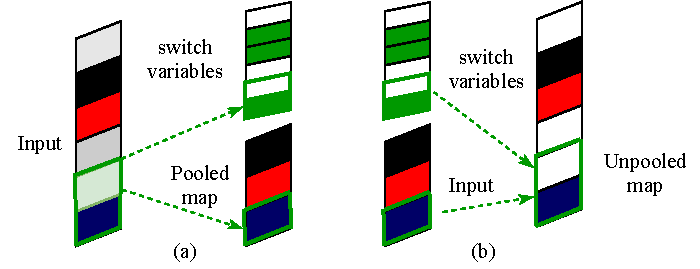
\includegraphics[width=0.6\textwidth]{sections/figures/pool_unpool.pdf}
    \caption{The model architecture. }
    \label{fig:model}
    \end{figure}
\end{center}
\subsection{The convolutional network}
Assembly code is selected as the input of the model. Based on previous studies, assembly instructions are more suitable for software fault prediction than other representations like software metrics and abstract syntax trees (ASTs) \cite{phan2017conv_asm}. Basically, software metrics simply capture surface features of programs, and ASTs just represent the program syntactic structures. While semantic bugs are more relevant to program behaviors than the structures \cite{viet2019transfer}. For this criterion, assembly code should be a selection because assembly instructions are translated into the machine code one by one. To feed into the network, each instruction is encoded as a real-valued vector with thirty dimensions. To learn the vector representations, we collected assembly instruction sequences from all experimental data and trained by the GloVe algorithm \cite{pennington2014glove}.   

\textbf{Vector representation} is the first layer of the networks. After obtaining instruction vectors, we form the lookup table $ E = e_1 \oplus e_2 \oplus ... \oplus e_N \in \mathbb{R}^{N \times d}$, where, $N$ is the number of unique assembly instructions and $d$ is the vector size; $e_i$ is the vector of $i^{th}$ instruction and $\oplus$ is the concatenation operation. Given an input program with instruction sequences $a_1, a_2, ..., a_L$, the embedding matrix is $E_p =  e_{idx(a_1)} \oplus e_{idx(a_2)} \oplus ... \oplus e_{idx(a_L)} \in \mathbb{R}^{L \times d} $,  in which $idx{(a_i)}$ is a mapping function returning the index of the assembly instruction $a_i$ in the lookup table.  
    \begin{center}
        \begin{figure}
        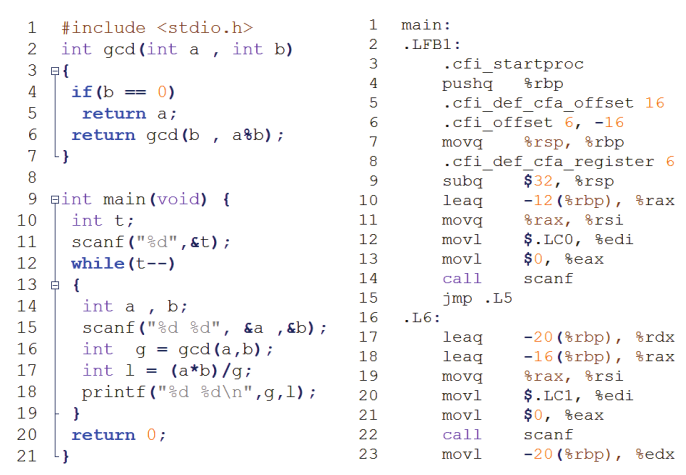
\includegraphics[width=\textwidth]{sections/figures/c2asm.png}
        \caption{A C code example and a snippet of its assembly instructions generated by GCC compiler.}
        \label{fig:c2asm}        
        \end{figure}
    \end{center}
\textbf{Convolutional layers} undertake the most important role in the network. These layers apply a set of filters sliding over sequences to learn local features. Specifically, the filters with sizes of 2 and 3 will capture the relations among 2 and 3 instructions, respectively. Stacking multiple convolutional layers make the network able to learn high-level abstract features and expand the local regions for feature extraction, but more difficult to train. Formally, given a input program with the embedding matrix $E_p =  e^p_1 \oplus e^p_2 \oplus ... \oplus e^p_L \in \mathbb{R}^{L \times d}$, a convolution will transform into a feature map with the same length $C^f =\{c^f_1, c^f_2, ..., c^f_L\}$:
    \begin{equation}
    c_i^f = f(W^f \cdot {e^p}_{i:i+h-1} + b_f)
    \end{equation}
    where $h$ is the filter size,
    $e^p_{i:i+h-1} = e^p_i \oplus e^p_{i+1} \oplus ... \oplus e^p_{i+h-1}$, $W_f \in \mathbb{R}^{h \times d}$, $f$ is an non-linear activation function, and $b_f$ is a bias.
Normally, many filters are used in a convolutional layer to extract features according to different relation aspects. 

\textbf{A pooling layer} is commonly stacked on each convolutional layer to perform dimension reduction. For high dimensional data, downsampling helps to reduce model parameters, and hence to speed up computational time and control overfitting. In the experimental datasets, a program may have up to 3,000 instructions resulting in a $3,000 \time 30$ embedding matrix. In addition, the convolution just transforms the input data without downsampling. Therefore, applying pooling layers is essential.

In pooling layers, each feature map is resized independently. Normally, a pooling layer splits a feature map into non-overlapping regions and then applies the pooling operation for such sub-regions. Two commonly used operations are $max$ and $average$. For example, a max pooling with the filter size of 2 and the stride of 2, the feature map column $C^f$ will be separated into two-value regions, and the greater one of each pair is selected. This results in the pool feature map with size of $L/2$. In the training process, the backward pass simply routes the gradient to the highest value in the forward pass. 

    \begin{center}
        \begin{figure}
        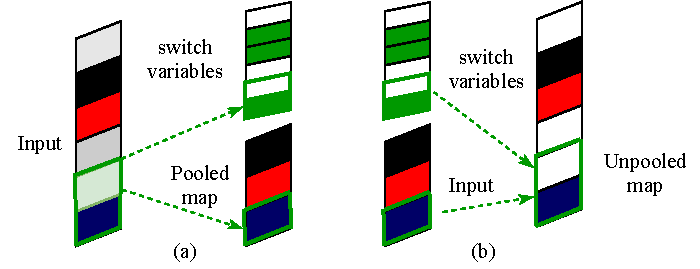
\includegraphics[width=\textwidth]{sections/figures/pool_unpool.pdf}
        \caption{Illustration of pooling (a) and unpooling (b) processes.}
        \label{fig:pool_unpool}        
        \end{figure}
    \end{center}
\subsection{The classifier}
For predicting faulty code, the classifier is built based on the features extracted by the convolutional network. This part includes a global pooling and some fully connected layers.

\textbf{Global pooling}. The last pooling layer in the part (1) is also a high dimensional features. To select the most sophisticated features, a global pooling is applied to pool each feature map into a single value.

\textbf{Fully connected layers} contains neurons that fully connect to all neurons in the previous layer. The activation of the last layer is $softmax$ to convert score values into distribution probabilities.
    \begin{equation}
    \label{eq:softmax}
        \sigma(\textbf{z}_c) = \frac{e^{z_c}}{\sum_{i = 1}^{K}{e^{z_i}}}
    \end{equation}
    where $K$ is the number of target labels, $c = 1, ..., K$, and $\textbf{z} = (z_1, ..., z_K)$

We use categorical cross-entropy to evaluate the classification loss. For an instance $i$, the loss is computed as follows:
    \begin{equation}
    \label{eq:loss_classification}
        L(y_i, \hat{y_i}) = -\sum_{c=1}^{K}{y_{i,c}log(p_{i,c})}
    \end{equation}{}
    where $y_{i,c}$ is the indicator function that has value of 1 if and only if $c$ is the correct target for the instance $i$. $p_{i,c}$ is the predicted probability for the class $c$ as in Equation \ref{eq:softmax}.
\subsection{The autoencoder}
An autoencoder consists of two segments, the encoder and the decoder (parts 1 and 3) that have symmetric structures. The encoder maps input sequences $\textbf{X}$ by function $\phi$ to latent representations $\textbf{F}$. Inversely, the decoder tries to recreate the original sequences $X$ by function $\psi$. The process can be formulated as follows.
    \begin{equation}
    \begin{split}
        &\phi : \textbf{X} \rightarrow \textbf{F} \\
        &\psi : \textbf{F} \rightarrow \textbf{X} \\
        &\phi, \psi = \underset{\phi, \psi}{\operatorname{argmin}}\left \| \textbf{X} - (\phi \circ  \psi)\textbf{X } \right \|^2    
    \end{split}
    \end{equation}

In the model, both the encoder and the decoder are built up from convolutional layers. A slight difference between the two architectures is that the pooling is used for dimension reduction in the encoder, while the decoder applies an upsampling to expand feature maps. 

The objective of training the autoencoder is to minimize the reconstruction errors. The loss function for an instance $x_i$ is as follows.
    \begin{equation}
    \label{eq:loss_reconstruction}
     \begin{split}
         L(x_i, {x_i}') &= \left \| x_i - {x_i}' \right \|^2 \\
                  &= \left \| x_i - \phi(\psi(x_i)) \right \|^2
    \end{split}
    \end{equation}
    where ${x_i}'$ is the reconstruction that has the same shape as $x_i$.
    
\subsection{Loss function}
The two branches shares the first part and are jointly trained. Therefore, the loss function of the whole model is the combination of classification and reconstruction errors. From equations \ref{eq:loss_classification} and \ref{eq:loss_reconstruction}, training process will minimize the following function.  
\begin{equation}
     \begin{split}
         L_i &= L(y_i, \hat{y_i}) + L(x_i, {x_i}') \\
             &= -\sum_{c=1}^{K}{y_{i,c}log(p_{i,c})} + \left \| x - \phi(\psi(x')) \right \|^2
    \end{split}
    \end{equation}
\section{Experiments}
\label{sec:experiments}
\subsection {Datasets}
To verify the model in terms of performance and the ability to learn with limited data, we used the datasets as in \cite{phan2017convolutional} to conduct experiments. Each dataset contains all source files written in C/C++ for solving a problem on CodeChef\footnote{\url{https://www.codechef.com/problems/<problem-name>}}, a contest site to learn programming languages. The collected problems are 1) SUMTRIAN for computing the sum of the numbers on the longest path in a triangular matrix, 2) FLOW016 for finding the greatest common divisor (GCD) and the least common multiple (LCM) of two integer numbers, 3) MNMX for finding the minimum cost to convert the array into a single element by several operations, 4) SUBINC for counting the non-decreasing subarrays in an array.

According to the execution result, a program is assigned to one of categories including \textit{0) clean code} if the output meets all the requirements, and defective code that result in \textit{1) time limit exceeded} - the running time is greater than the time limit, \textit{2) wrong answer} - the output does not match with the expected, \textit{3) runtime error} - the execution process was interrupted, and \textit{4) syntax error} - the compilation was failed.         

Table~\ref{table:datastatistics} shows data statistics on the experimental datasets. As can be seen, all the datasets are unbalanced in which the instance numbers of classes 0 and 1 dominate those the other classes. We used the same data split as in \cite{phan2017convolutional} with the training, validation and testing ratio of 3:1:1.
\begin{table}[]
\centering
\setlength{\tabcolsep}{4pt}
\caption{The statistics on the number of samples for the datasets}
\label{table:datastatistics}
\begin{tabular}{lrrrrrr}
\hline
Dataset & Total & Class 0 & Class 1 & Class 2 & Class 3 & Class 4 \\ \hline
FLOW016 &10,648 &3,472 &4,165 &231 &2,368 &412 \\
MNMX    &8,745 &5,157 &3,073 &189 &113 &213 \\
SUBINC  &6,484&3,263&2,685&206&98&232\\
SUMTRIAN&21,187&9,132&6,948&419&2,701&1,987\\ \hline
\end{tabular}
\end{table}

\subsection{Baselines and training scenarios}
\textbf{Baselines}. We compare our proposed method with a convolutional neural network (CNN) (as the classification branch without the autoencoder), and the CNN with transfer learning. As confirmed in many studies \cite{phan2017convolutional,phan2018dgcnn, phan2017conv_asm}, assembly code-based methods reach much higher performance than those based on software metrics and ASTs on these datasets. In addition, transfer learning has proved as a good solution for limited data in various areas such as image, speech, and language processing \cite{weiss2016survey}. Thus, two baselines including the CNN trained from scratch and the CNN with transfer learning are selected to verify the proposed model performance.

\textbf{Training scenarios}. To assess the influence of data amount on the learning ability, we trained the models with 100\%, 75\%, 50\%, and 25\% of the training set and ran prediction for the whole validation and test sets.

To judge the contribution of the autoencoder, the proposed model is trained with three scenarios as follows.
\begin{itemize}
    \item AE\-CNN: We first train the autoencoder and then remain the weights for the part 1 of convolutions to train CNN independently. This can be considered as a type of self-transfer learning because we initialize the weights using the same data but without target label information.
    \item CNN\-Mul: the autoencoder and CNN are trained simultaneously from scratch.
    \item AE\-CNN\-Mul: The autoencoder is pretrained and then we continue training the whole model. 
\end{itemize}

For transfer learning, we merge all data of the other problems to pretrain the CNN and then reuse the network weights as the initialization to build the classifier for the current problem.  
\subsection {Evaluation Measures}
We used three common used measures including accuracy, F1 and AUC (the area under the receiver operating characteristic \- ROC) to evaluate model performance. The accuracy, and F1 can be computed from the confusion matrix constructed from the prediction results. For binary classification where a sample belongs one of two categories +1 (positive) and -1 (negative), the confusion matrix is as follows.
\begin{table}[]
\begin{center}
\caption{The confusion matrix}
\begin{tabular}{llcc}
\hline
 & & \multicolumn{2}{c}{Predicted} \\ \cline{3-4} 
 &  & +1 (Positive) & -1 (Negative) \\ \hline
\multirow{2}{*}{Actual} & \multicolumn{1}{c}{+1} & TP & FN  \\
                        & \multicolumn{1}{c}{-1} & FP & TN  \\ \hline
\end{tabular}
\end{center}
\end{table}

Classification accuracy:
\begin{equation}
    Accuracy = \frac{TP + TN}{TP + TN + FP + FN}
\end{equation}
The F1 measure:
\begin{equation}
    F1 = \frac{2* Recall * Precision}{Recall + Precision}
\end{equation}
where $Precision = \frac{TP}{TP + FP}$ and $Recall = \frac{TP}{TP + FN}$

AUC is an essential measure to evaluate classifiers, especially in cases of unbalance data. AUC is the area under the ROC curve that is generated by plotting all points of (true positive rate $TPR = \frac{TP}{P}$ , the false positive rate $FPR = \frac{FP}{N}$) at different discrimination thresholds. The AUC shows the ability to distinguish between classes.

The above measures were presented for binary classifiers. To extend to multi-class problems, the measures are computed by several ways:
\begin{itemize}
    \item micro. computing the TPR, and FPR, FP and TP globally.
    \item macro. computing the metrics for each class and take the unweighted mean.
    \item weighted. Similar to the macro, but taking the weighted mean according to the number of instances for each class. 
\end{itemize}{}

\section{Result Analysis and Discussion}
\label{sec:results}
From Table \ref{tab:results}, it should be confirmed that finding solutions to deal with the data shortage is critical. Indeed, the CNN downgrades significantly when we reduce the amount of training data from 100\% to 25\%. Specifically, the AUC of CNN decreases 5\%, 9\%, \%6, and 2\% on FLOW016, MNMX, SUBINC, and SUMTRIAN, respectively. This issue also happens in the cases of Accuracy and F1. Unlikely, transferable models work more stable with less data. Taking the 25\% data as an example, the pretraining the autoencoder in the multitask model (AE\_CNN\_Mul) achieves the highest performance on all the datasets.             

In terms of dealing with limited data, our proposed models outperforms transfer learning.  

Less sensitive

Considering the ability to distinguish among faulty types, 

Good representation



...Fig. \ref{fig:auc} shows ... Fig. \ref{fig:visualize} shows...

\begin{table*}[ht]
\centering
\caption{The comparison of the methods according to Accuracy, F1, and AUC. Each row block shows the classification performance for the use of 100\%, 75\%, 50\%, and 25\% of labelled training data. Each cell is in the form of mean $\pm$ standard deviation for 5 times of running.}
\label{tab:results}
\begin{adjustbox}{width=\textwidth}
% Please add the following required packages to your document preamble:
% \usepackage{multirow}
\begin{tabular}{lcccccccccccc}
\hline
\multirow{2}{*}{Approach} & \multicolumn{3}{c}{FLOW016}                                    & \multicolumn{3}{c}{MNMX}                                       & \multicolumn{3}{c}{SUBINC}                                     & \multicolumn{3}{c}{SUMTRIAN}                                   \\ \cline{2-13} 
                          & Acc.                & F1                  & AUC                & Acc.                & F1                  & AUC                & Acc.                & F1                  & AUC                & Acc.                & F1                  & AUC                \\ \hline
\textbf{100}&&&&&&&&&&&& \\
CNN                  & 72.52$\pm$0.23          & 71.34$\pm$0.15          & 0.80$\pm$0.08          & 81.99$\pm$0.06          & 80.03$\pm$0.21          & 0.80$\pm$0.02          & 70.93$\pm$0.71          & 69.94$\pm$0.32          & 0.72$\pm$0.11          & 67.97$\pm$0.34          & 66.35$\pm$0.42          & 0.77$\pm$0.19          \\
CNN\_Trans        & 73.05$\pm$0.54          & 71.67$\pm$0.43          & 0.81$\pm$0.34          & 81.53$\pm$0.31          & 79.07$\pm$0.55          & 0.80$\pm$0.11          & 69.08$\pm$0.92          & 68.15$\pm$0.81          & 0.74$\pm$0.52          & 67.12$\pm$0.73          & 66.06$\pm$0.56          & 0.79$\pm$0.11          \\
AE\_CNN              & \textbf{74.83$\pm$0.25} & 72.92$\pm$0.21          & 0.81$\pm$0.10          & \textbf{83.43$\pm$0.31} & \textbf{81.44$\pm$0.37} & \textbf{0.81$\pm$0.28} & 72.59$\pm$0.66          & \textbf{71.62$\pm$0.28} & 0.73$\pm$0.38          & \textbf{68.09$\pm$0.87} & \textbf{67.33$\pm$0.51} & 0.78$\pm$0.21 \\
CNN\_Mul       & 73.90$\pm$0.32          & 72.55$\pm$0.33          & 0.80$\pm$0.12          & 82.11$\pm$0.29          & 81.05$\pm$0.08          & 0.80$\pm$0.12          & 71.47$\pm$0.82          & 70.32$\pm$0.41          & 0.73$\pm$0.41          & 66.66$\pm$0.63          & 65.69$\pm$0.66          & 0.78$\pm$0.58          \\
AE\_CNN\_Mul   & 73.96$\pm$0.18          & \textbf{73.06$\pm$0.11} & \textbf{0.82$\pm$0.07} & 83.06$\pm$0.23          & 81.12$\pm$0.10          & 0.80$\pm$0.03          & \textbf{72.63$\pm$0.59} & 71.40$\pm$0.25          & \textbf{0.74$\pm$0.22} & 67.53$\pm$0.81          & 66.54$\pm$0.47          & \textbf{0.79$\pm$0.17} \\ \hline
\textbf{75}&&&&&&&&&&&& \\
CNN                   & 71.95$\pm$0.33          & 70.40$\pm$0.31          & 0.78$\pm$0.53          & 79.96$\pm$0.23          & 78.62$\pm$0.73          & 0.78$\pm$0.70          & 70.62$\pm$0.55          & 69.99$\pm$0.52          & 0.72$\pm$0.11          & 65.99$\pm$0.48          & 64.9$\pm$0.33           & 0.78$\pm$0.22          \\
CNN\_Trans         & 72.91$\pm$0.41          & 71.73$\pm$0.39          & 0.81$\pm$0.27          & 79.04$\pm$0.62          & 77.52$\pm$0.24          & 0.76$\pm$0.22          & 67.77$\pm$0.67          & 66.24$\pm$0.66          & 0.70$\pm$0.23          & 66.89$\pm$0.24          & 66.20$\pm$0.19          & 0.78$\pm$0.30          \\
AE\_CNN               & 72.82$\pm$0.31          & 71.86$\pm$0.21          & 0.80$\pm$0.10          & \textbf{81.41$\pm$0.29} & \textbf{78.89$\pm$0.58} & 0.78$\pm$0.08          & 71.55$\pm$0.49          & 70.14$\pm$0.43          & \textbf{0.74$\pm$0.10} & 66.07$\pm$0.67          & 64.34$\pm$0.41          & 0.78$\pm$0.32          \\
CNN\_Mul        & 72.79$\pm$0.41          & 71.19$\pm$0.42          & 0.79$\pm$0.09          & 80.11$\pm$0.58          & 78.12$\pm$0.65          & 0.78$\pm$0.82          & 71.16$\pm$0.50          & 69.59$\pm$0.45          & 0.72$\pm$0.32          & 65.43$\pm$0.42          & 63.84$\pm$0.23          & 0.78$\pm$0.15          \\
AE\_CNN\_Mul    & \textbf{73.74$\pm$0.21} & \textbf{72.78$\pm$0.11} & \textbf{0.81$\pm$0.12} & 81.02$\pm$0.56          & 78.80$\pm$0.71          & \textbf{0.79$\pm$0.12} & \textbf{71.67$\pm$0.38} & \textbf{70.44$\pm$0.25} & 0.72$\pm$0.26          & \textbf{67.77$\pm$0.72} & \textbf{66.18$\pm$0.37} & \textbf{0.79$\pm$0.09} \\ \hline
\textbf{50}&&&&&&&&&&&& \\
CNN                   & 70.08$\pm$0.92          & 70.12$\pm$0.65          & 0.77$\pm$0.16          & 78.80$\pm$0.11          & 77.22$\pm$0.81          & \textbf{0.77$\pm$0.62} & 68.79$\pm$0.87          & 67.17$\pm$0.33          & \textbf{0.70$\pm$0.34} & 64.32$\pm$0.15          & 62.78$\pm$0.32          & 0.76$\pm$0.17          \\
CNN\_Trans         & 72.53$\pm$0.82          & 71.22$\pm$0.77          & 0.79$\pm$0.20          & 77.84$\pm$0.79          & 76.54$\pm$0.55          & 0.76$\pm$0.78          & 65.76$\pm$0.71          & 64.92$\pm$0.67          & 0.68$\pm$0.22          & 65.77$\pm$0.81          & 64.14$\pm$0.72          & 0.77$\pm$0.53          \\
AE\_CNN               & 71.98$\pm$0.47          & 71.02$\pm$0.31          & 0.78$\pm$0.21          & \textbf{80.11$\pm$0.77} & \textbf{78.09$\pm$0.68} & \textbf{0.77$\pm$0.54} & \textbf{70.16$\pm$0.20} & 67.87$\pm$0.45          & \textbf{0.70$\pm$0.15} & \textbf{66.21$\pm$0.46} & \textbf{64.75$\pm$0.23} & \textbf{0.78$\pm$0.21} \\
CNN\_Mul        & 70.29$\pm$0.31          & 70.56$\pm$0.50          & 0.78$\pm$0.32          & 78.99$\pm$0.18          & 76.12$\pm$0.82          & 0.76$\pm$0.81          & 68.02$\pm$0.23          & 66.92$\pm$0.24          & 0.69$\pm$0.36          & 64.18$\pm$0.51          & 61.78$\pm$0.40          & 0.76$\pm$0.19          \\
AE\_CNN\_Mul    & \textbf{72.69$\pm$0.52} & \textbf{71.19$\pm$1.22} & \textbf{0.80$\pm$0.01} & 79.55$\pm$0.61          & 77.80$\pm$0.77          & \textbf{0.77$\pm$0.15} & 69.25$\pm$0.81          & \textbf{68.84$\pm$0.44} & \textbf{0.70$\pm$0.39} & 64.98$\pm$0.74          & 63.8$\pm$0.88           & 0.77$\pm$0.39          \\ \hline
\textbf{25}&&&&&&&&&&&& \\
CNN                   & 68.98$\pm$0.61          & 67.82$\pm$0.33          & 0.75$\pm$0.16          & 77.56$\pm$0.73          & 76.32$\pm$0.78          & 0.71$\pm$0.21          & 65.54$\pm$0.16          & 63.06$\pm$0.46          & 0.66$\pm$0.27          & 62.12$\pm$0.71          & 60.07$\pm$0.66          & 0.74$\pm$0.26          \\
CNN\_Trans         & 69.11$\pm$0.22          & 68.12$\pm$0.15          & \textbf{0.77$\pm$0.52} & 76.10$\pm$.082          & 75.08$\pm$0.66          & 0.72$\pm$0.15          & 62.07$\pm$0.52          & 59.58$\pm$0.46          & 0.64$\pm$0.25          & \textbf{64.82$\pm$0.57} & \textbf{62.44$\pm$0.33} & \textbf{0.76$\pm$0.25} \\
AE\_CNN               & 69.15$\pm$0.36          & 68.02$\pm$0.41          & 0.76$\pm$0.06          & \textbf{79.24$\pm$0.81} & \textbf{76.59$\pm$0.65} & \textbf{0.73$\pm$0.11} & 66.11$\pm$0.90          & 63.71$\pm$0.61          & 0.66$\pm$0.61          & 62.51$\pm$0.62          & 60.27$\pm$0.55          & 0.74$\pm$0.31          \\
CNN\_Mul        & 68.92$\pm$0.44          & 67.75$\pm$0.53          & 0.76$\pm$0.73          & 77.01$\pm$0.77          & 76.11$\pm$0.81          & \textbf{0.73$\pm$0.72} & 65.65$\pm$0.86          & 63.66$\pm$0.52          & 0.66$\pm$0.15          & 61.32$\pm$0.79          & 60.57$\pm$0.92          & 0.75$\pm$0.29          \\
AE\_CNN\_Mul    & \textbf{69.75$\pm$0.38} & \textbf{68.21$\pm$0.33} & \textbf{0.77$\pm$0.33} & 78.08$\pm$0.18          & 76.12$\pm$0.66          & \textbf{0.73$\pm$0.64} & \textbf{67.31$\pm$0.71} & \textbf{64.07$\pm$0.44} & \textbf{0.68$\pm$0.29} & 64.75$\pm$0.53          & 62.20$\pm$0.51          & \textbf{0.76$\pm$0.39} \\ \hline
\end{tabular}
\end{adjustbox}
\end{table*}

\begin{figure}[]
  \centering
%    \vfill %\vspace{-0.4cm}
  \subfloat[]{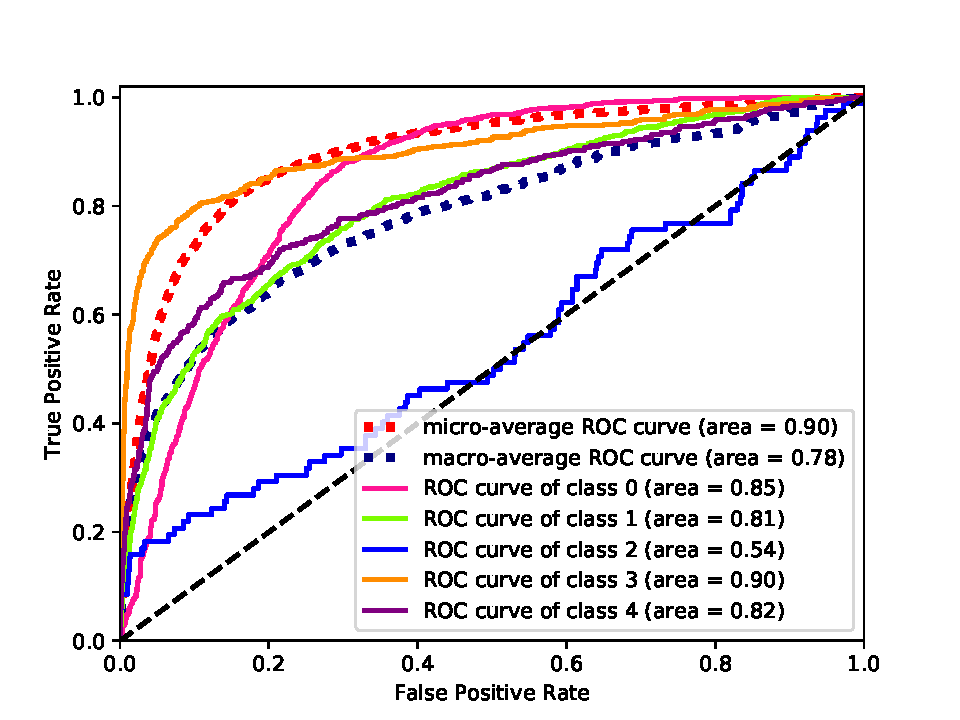
\includegraphics[width=6cm]{sections/figures/cnn_SUMTRIAN_100.pdf}\label{fig:auc_cnn_sum}}
  \hfill %\vspace{-0.4cm}
  \subfloat[]{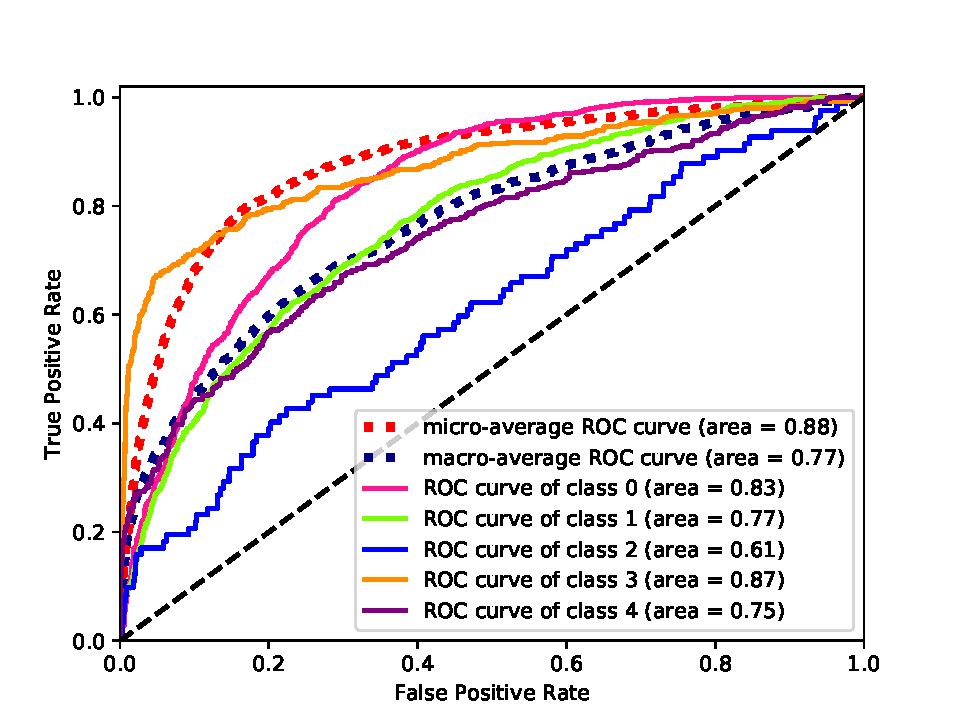
\includegraphics[width=6cm]{sections/figures/ae_cnn_multitask_SUMTRIAN_25.pdf}\label{fig:auc_ae_cnnmul_sum}}
  \caption{The ROC curves on the SUMTRIAN test set of the CNN trained with 100\% data (Fig.~\ref{fig:auc_cnn_sum}) and AE\_CNN\_Mul trained with 25\% data (Fig.~\ref{fig:auc_ae_cnnmul_sum}).}
 \label{fig:auc_sum}
\end{figure}

\begin{figure}[]
  \centering
%    \vfill %\vspace{-0.4cm}
  \subfloat[]{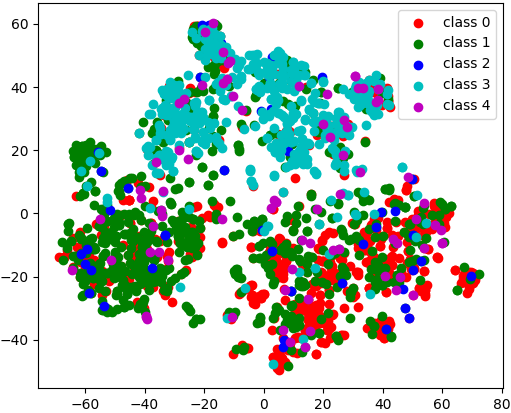
\includegraphics[width=6cm]{sections/figures/cnn_FLOW016_100_visualize.png}\label{fig:fea_cnn_flow}}
  \hfill %\vspace{-0.4cm}
  \subfloat[]{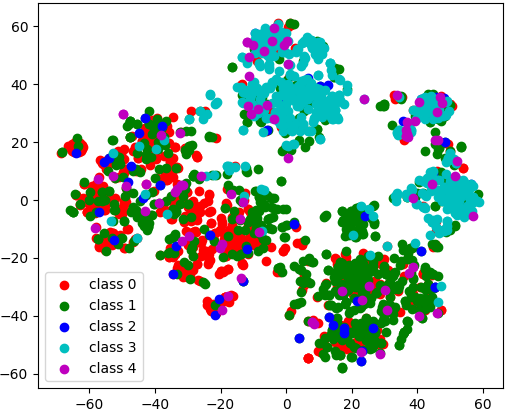
\includegraphics[width=6cm]{sections/figures/ae_cnn_FLOW016_100_visualize.png}\label{fig:fea_ae_cnn_flow}}
   \vfill %\vspace{-0.4cm}
    \subfloat[]{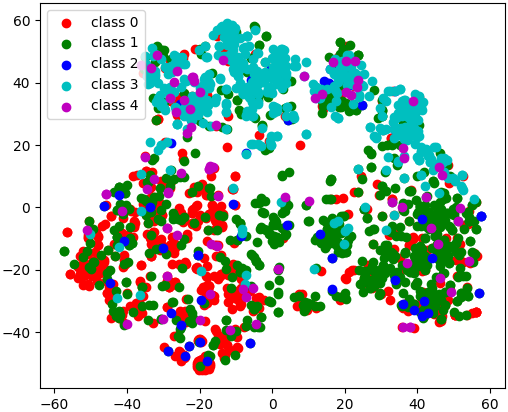
\includegraphics[width=6cm]{sections/figures/cnn_multi_task_FLOW016_100_visualize.png}\label{fig:fea_cnn_mul_flow}}
  \hfill %\vspace{-0.4cm}
  \subfloat[]{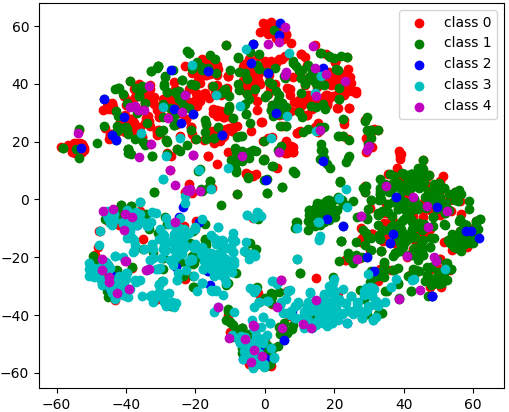
\includegraphics[width=6cm]{sections/figures/ae_cnn_multitask_FLOW016_100_visualize.png}\label{fig:fea_ae_cnn_mul_flow}}
  \caption{Feature visualization on the FLOW016 test set of methods CNN (Fig. \ref{fig:fea_cnn_flow}), AE\_CNN (Fig. \ref{fig:fea_cnn_flow}), CNN\_Mul (Fig. \ref{fig:fea_cnn_flow}), and AE\_CNN\_Mul (Fig. \ref{fig:fea_cnn_flow})}
 \label{fig:fea_flow016}
\end{figure}


\begin{figure}[]
  \centering
%    \vfill %\vspace{-0.4cm}
  \subfloat[]{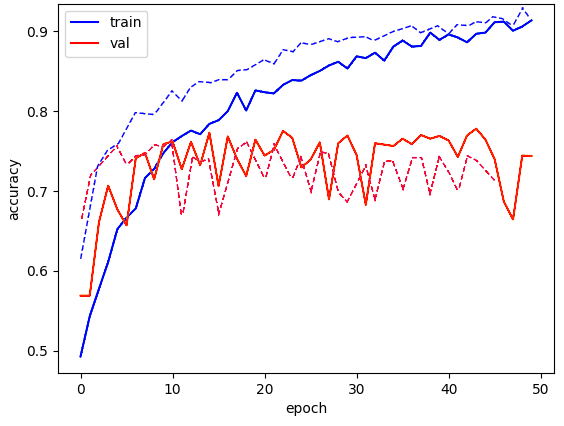
\includegraphics[width=6cm]{sections/figures/MNMX_25_train_valid_acc.png}\label{fig:mnmx_25_train_valid_acc}}
  \hfill %\vspace{-0.4cm}
  \subfloat[]{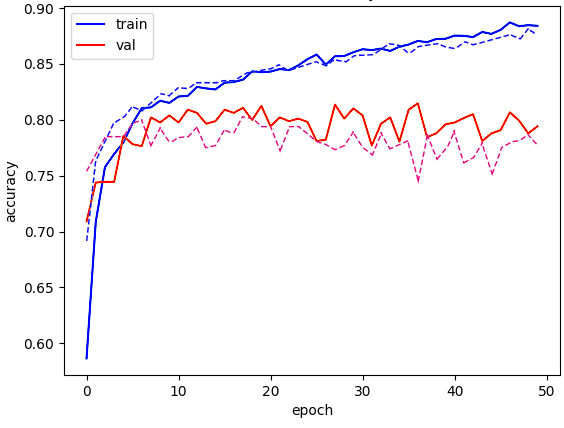
\includegraphics[width=6cm]{sections/figures/MNMX_100_train_valid_acc.png}\label{fig:mnmx_100_train_valid_acc}}
  \caption{The training process of AE\_CNN\_Mul (solid lines) and CNN\_Trans (dashed lines) classifiers on MNMX with 25\% (\ref{fig:mnmx_25_train_valid_acc}) and 100\% (\ref{fig:mnmx_100_train_valid_acc}) data.}
 \label{fig:mnmx_training_process}
\end{figure}

\section{Conclusion}
\label{sec:conclusion}
\section*{Acknowledgements}
This research is funded by the Vietnam National Foundation for Science and Technology Development (NAFOSTED) under grant number 102.05-2018.306.
\section*{References}

\bibliography{refs}

\end{document}